%%%%
\section{Poluição do Ar}

Poluição do ar resulta de uma complexa mistura de emissões naturais e 
antropogênicas, estima-se que a poluição do ar é responsável por 
$3,2$ milhões de mortes por ano no mundo todo \cite{lim2013}.

A inalação de material particulado exerce um papel importante na 
exacerbação de doenças respiratórias, incluindo enfisema pulmonar e asma. 
Suas pequenas dimensões e massa, facilitam a penetração do MP no sistema 
respiratório, trazendo danos aos alvéolos pulmonares. 
Nas áreas danificadas ocorre o comprometimento das 
trocas gasosas podendo, também, acarretar problemas cardiovasculares
\cite{arbex2012}.

%%%%
\subsection{Material Particulado $MP$ ou Aerossol Atmosférico}

Os Material Particulado $MP$ ou  Aerossóis Atmosféricos são partículas
sólidas ou líquidas em suspensão em um gás, as quais tem diâmetro 
aerodinâmico compreendido  entre $0,001-100\mu m$. 
A parte considerada inalável para humanos tem diâmetro menor que 10 $\mu m$
e se comporta praticamente como gás.

As partículas maiores que 10 $\mu m$ têm dificuldade em penetrar 
no sistema respiratório porque seu arraste pelo ar inalado não vence 
a força da gravidade \cite{seinfeld1998}.

O $MP$ pode ser classificado por tamanho, formação 
(primária ou secundária), composição química, remoção da atmosfera ou 
forma da partículas \citep{seinfeld1998}.

Esquema que mostra os processo de formação 

\begin{itemize}
  \item \textbf{moda ultra-fina:} são oriundas de processos mecânicos como fragmentação, 
        movimentação e manuseio. Partículas grossas são removidas da atmosfera 
        por sedimentação.
  \item \textbf{moda nucleação:} núcleo de condensação são criados devido a 
        condensação de vapores quentes ou durante o processo de 
        transformação de gás em partícula. Partículas formadas por 
        nucleação são removidas da atmosfera por aglomeração. 
        Essa moda ainda pode ser subdividida em \textbf{partículas ultra-finas} e 
        \textbf{núcleos de Aitken}.  
  \item \textbf{moda acumulação:} partículas na moda de acumulação são criadas 
         a partir de núcleos de condensação através da coagulação ou 
         condensação de vapores. Partículas formadas por acumulação
         são removidas da atmosfera por deposição seca ou úmida.
  \item \textbf{moda grossa:} são oriundas de processos mecânicos como fragmentação, 
        movimentação e manuseio. Partículas grossas são removidas da atmosfera 
        por sedimentação.
\end{itemize}

\begin{figure}[H]
\begin{center}
  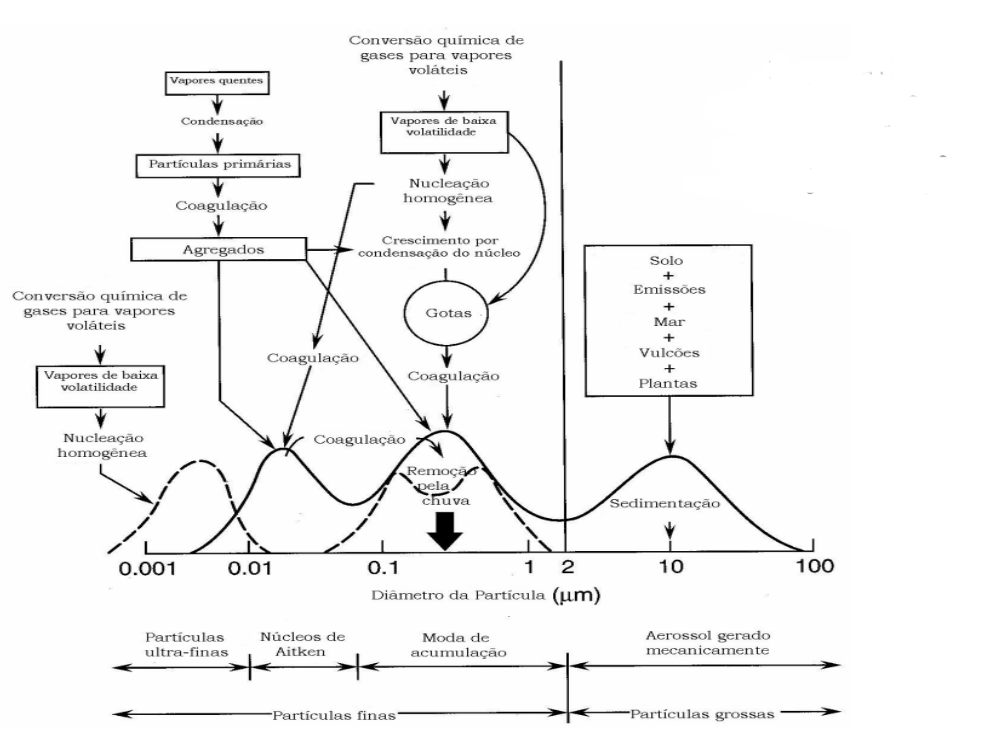
\includegraphics[width=0.5\textwidth]{../inputs/images/modas_aerossol.png}
  \caption{Esquema da distribuição de tamanho do aerossol atmosférico 
           \cite{finlayson1999} \label{fig:modas_aerossol}}
\end{center}
\end{figure}

O material particulado fino $MP_{2,5}$ engloba a moda de nucleação e acumulação e
o material particulado grosso $MP_{2,5-10}$ somente a moda grossa. 

O $MP_{2,5-10}$ tende a ficar retido na parte superior do sistema respiratório, 
enquanto que $MP_{2,5}$ tem maior facilidade para penetrar e atingir os alvéolos pulmonares, 
podendo comprometer significativamente a saúde humana. 

O $MP$ pode ser emitido por diferentes fontes antropogênicas ou naturais e, 
também, pode ser gerado secundariamente na atmosfera por reações químicas. 
Fontes potenciais como queimadas, indústrias e veículos automotivos, particularmente,
emitem a maior parte dos poluentes urbanos.

Na moda fina encontra-se principalmente íons $SO_4^=$, 
íons $ NO_3^-$, carbono elementar, carbono orgânico, compostos orgânicos elementar
condensados, metais (cádmio, níquel, vanádio, zinco, cromo, ferro, mercúrio), 
sulfatos, nitratos, nitrato amônia \cite{finlayson1999}. 

O oxido de nitrogênio (NOx) e amônia NH3 formam nitrato de amônio e 
o dióxido de enxofre (SO2) e amônia NH3 formam o sulfato de amônio, 
portanto são secundário.

Na moda grossa encontra-se principalmente: poeira de solo, fuligem, 
pólen, Si, Al, ferro, K, Ca e metais alcalinos.

%%%%
\section{Saúde}

A deposição no sistema respiratório humano ocorre em função do diâmetro da partícula.
As partículas mais finas chegam nos bronquíolos e as maiores só alcançam os alvéolos.
As maiores ficam no nariz (traqueobrônquica) nasofaringe. 
Os vírus são $MP_{2,5}$ e bactérias são $MP_{10}$. 

O próprio corpo consegue remover partículas através do Macrófago alveolar 
e do sistema linfático. 

%%%%
\section{Meio Ambiente}
Ao depositar em folhas, as partículas impedem a absorção de luz. 

Efeitos na visibilidade.

Efeitos na formação de nuvens.


